% vim: set spell spelllang=en tw=100 et sw=4 sts=4 foldmethod=marker foldmarker={{{,}}} :

\documentclass{beamer}

\usepackage{tikz}
\usepackage{xcolor}
\usepackage{complexity}
\usepackage{hyperref}
\usepackage{microtype}
\usepackage{amsmath}                   % \operatorname
\usepackage{amsfonts}                  % \mathcal
\usepackage{amssymb}                   % \nexists
\usepackage[vlined]{algorithm2e} % algorithms
\usepackage{centernot}
\usepackage{listings}
\usepackage{csquotes}
\usepackage{fancyvrb}
\usepackage{bussproofs}
\usepackage{multicol}
\usepackage{booktabs}
\usepackage{mathtools}
\usepackage{pifont}
\usepackage{marvosym}
\usepackage{cancel}

\RequirePackage[tt=false, type1=true]{libertine}
\RequirePackage[varqu]{zi4}
\RequirePackage[libertine]{newtxmath}
\RequirePackage[T1]{fontenc}

\usetikzlibrary{shapes, arrows, shadows, calc, positioning, fit}
\usetikzlibrary{decorations.pathreplacing, decorations.pathmorphing, shapes.misc}
\usetikzlibrary{tikzmark, backgrounds}
\usetikzlibrary{trees, overlay-beamer-styles}

\definecolor{uofguniversityblue}{rgb}{0, 0.219608, 0.396078}
\definecolor{uofgheather}{rgb}{0.356863, 0.32549, 0.490196}
\definecolor{uofgaquamarine}{rgb}{0.603922, 0.72549, 0.678431}
\definecolor{uofgslate}{rgb}{0.309804, 0.34902, 0.380392}
\definecolor{uofgrose}{rgb}{0.823529, 0.470588, 0.709804}
\definecolor{uofgmocha}{rgb}{0.709804, 0.564706, 0.47451}
\definecolor{uofgsandstone}{rgb}{0.321569, 0.278431, 0.231373}
\definecolor{uofgforest}{rgb}{0, 0.2, 0.129412}
\definecolor{uofglawn}{rgb}{0.517647, 0.741176, 0}
\definecolor{uofgcobalt}{rgb}{0, 0.615686, 0.92549}
\definecolor{uofgturquoise}{rgb}{0, 0.709804, 0.819608}
\definecolor{uofgsunshine}{rgb}{1.0, 0.862745, 0.211765}
\definecolor{uofgpumpkin}{rgb}{1.0, 0.72549, 0.282353}
\definecolor{uofgthistle}{rgb}{0.584314, 0.070588, 0.447059}
\definecolor{uofgrust}{rgb}{0.603922, 0.227451, 0.023529}
\definecolor{uofgburgundy}{rgb}{0.490196, 0.133333, 0.223529}
\definecolor{uofgpillarbox}{rgb}{0.701961, 0.047059, 0}
\definecolor{uofglavendar}{rgb}{0.356863, 0.301961, 0.580392}

% {{{ theme things
\useoutertheme[footline=authortitle]{miniframes}
\useinnertheme{rectangles}

\setbeamerfont{block title}{size={}}
\setbeamerfont{title}{size=\large,series=\bfseries}
\setbeamerfont{section title}{size=\large,series=\mdseries}
\setbeamerfont{author}{size=\normalsize,series=\mdseries}
\setbeamercolor*{structure}{fg=uofguniversityblue}
\setbeamercolor*{palette primary}{use=structure,fg=black,bg=white}
\setbeamercolor*{palette secondary}{use=structure,fg=white,bg=uofgcobalt}
\setbeamercolor*{palette tertiary}{use=structure,fg=white,bg=uofguniversityblue}
\setbeamercolor*{palette quaternary}{fg=white,bg=black}
\setbeamercolor{block body}{bg=structure!10}
\setbeamercolor{block title}{bg=structure,fg=white}
\setbeamertemplate{blocks}[rounded]
\setbeamercolor*{titlelike}{parent=palette primary}

\beamertemplatenavigationsymbolsempty

\setbeamertemplate{title page}
{
    \begin{tikzpicture}[remember picture, overlay]
        \node at (current page.north west) {
            \begin{tikzpicture}[remember picture, overlay]
                \fill [fill=uofguniversityblue, anchor=north west] (0, 0) rectangle (\paperwidth, -3.0cm);
            \end{tikzpicture}
        };

        \node (logo) [anchor=north east, shift={(-0.6cm,-0.2cm)}] at (current page.north east) {
            
\includegraphics[keepaspectratio=true,scale=0.5]{../../images/UoG_keyline.pdf}
        };

        \node (logo2) [anchor=north, below=0.2cm of logo.south] {
            
\includegraphics[keepaspectratio=true,scale=0.1]{../../images/RAEngWhite.pdf}
        };

        \coordinate (logos) at ($(logo.south)!0.5!(logo2.north)$);

        \node [anchor=west, xshift=0.2cm] at (current page.west |- logos) {
            \begin{minipage}{0.65\paperwidth}\raggedright
                {\usebeamerfont{title}\usebeamercolor[white]{}\inserttitle}\\[0.2cm]
                {\usebeamerfont{author}\usebeamercolor[white]{}\insertauthor}\\[0.2cm]
                {\usebeamerfont{author}\usebeamercolor[white]{}\tiny With numerous co-conspirators, including Bart Bogaerts, Jan Elffers, \\
                Stephan Gocht, Ross McBride, Matthew McIlree, Jakob Nordstr{\"o}m, \\
                Andy Oertel, Patrick Prosser, and James Trimble \\[0cm]}
            \end{minipage}
        };
    \end{tikzpicture}
}

\setbeamertemplate{section page}
{
    \begin{centering}
        \begin{beamercolorbox}[sep=12pt,center]{part title}
            \usebeamerfont{section title}\insertsection\par
        \end{beamercolorbox}
    \end{centering}
}

\newcommand{\frameofframes}{/}
\newcommand{\setframeofframes}[1]{\renewcommand{\frameofframes}{#1}}

\makeatletter
\setbeamertemplate{footline}
{%
    \begin{beamercolorbox}[colsep=1.5pt]{upper separation line foot}
    \end{beamercolorbox}
    \begin{beamercolorbox}[ht=2.5ex,dp=1.125ex,%
        leftskip=.3cm,rightskip=.3cm plus1fil]{author in head/foot}%
        \leavevmode{\usebeamerfont{author in head/foot}\insertshortauthor}%
        \hfill%
        {\usebeamerfont{institute in head/foot}\usebeamercolor[fg]{institute in head/foot}\insertshortinstitute}%
    \end{beamercolorbox}%
    \begin{beamercolorbox}[ht=2.5ex,dp=1.125ex,%
        leftskip=.3cm,rightskip=.3cm plus1fil]{title in head/foot}%
        {\usebeamerfont{title in head/foot}\insertshorttitle}%
        \hfill%
        {\usebeamerfont{frame number}\usebeamercolor[fg]{frame number}\insertframenumber~\frameofframes~\inserttotalframenumber}
    \end{beamercolorbox}%
    \begin{beamercolorbox}[colsep=1.5pt]{lower separation line foot}
    \end{beamercolorbox}
}

\makeatletter
\newenvironment{nearlyplainframe}[2][]{
    \def\beamer@entrycode{\vspace*{-\headheight}\vspace*{3pt}}
    \setbeamertemplate{headline}
    {%
        \begin{beamercolorbox}[colsep=1.5pt]{upper separation line head}
        \end{beamercolorbox}
        \begin{beamercolorbox}[ht=0.5ex,dp=0.125ex,%
            leftskip=.3cm,rightskip=.3cm plus1fil]{title in head/foot}%
        \end{beamercolorbox}%
        \begin{beamercolorbox}[ht=0.5ex,dp=0.125ex,%
            leftskip=.3cm,rightskip=.3cm plus1fil]{author in head/foot}%
        \end{beamercolorbox}%
        \begin{beamercolorbox}[colsep=1.5pt]{lower separation line head}
        \end{beamercolorbox}
        \vspace*{\headheight}
    }

    \setbeamertemplate{footline}
    {%
        \begin{beamercolorbox}[colsep=1.5pt]{upper separation line foot}
        \end{beamercolorbox}
        \begin{beamercolorbox}[ht=0.5ex,dp=0.125ex,%
            leftskip=.3cm,rightskip=.3cm plus1fil]{author in head/foot}%
        \end{beamercolorbox}%
        \begin{beamercolorbox}[ht=0.5ex,dp=0.125ex,%
            leftskip=.3cm,rightskip=.3cm plus1fil]{title in head/foot}%
        \end{beamercolorbox}%
        \begin{beamercolorbox}[colsep=1.5pt]{lower separation line foot}
        \end{beamercolorbox}
    }

    \begin{frame}[#1]{#2}
    }{
    \end{frame}
}
\makeatother

\makeatletter
\newenvironment{justborderframe}[2][]{
    \def\beamer@entrycode{\vspace*{-\headheight}}
    \setbeamertemplate{headline}
    {%
        \begin{beamercolorbox}[colsep=1.5pt]{upper separation line head}
        \end{beamercolorbox}
        \begin{beamercolorbox}[ht=0.5ex,dp=0.125ex,%
            leftskip=.3cm,rightskip=.3cm plus1fil]{title in head/foot}%
        \end{beamercolorbox}%
        \begin{beamercolorbox}[ht=0.5ex,dp=0.125ex,%
            leftskip=.3cm,rightskip=.3cm plus1fil]{author in head/foot}%
        \end{beamercolorbox}%
        \begin{beamercolorbox}[colsep=1.5pt]{lower separation line head}
        \end{beamercolorbox}
        \vspace*{\headheight}
    }

    \setbeamertemplate{footline}
    {%
        \begin{beamercolorbox}[colsep=1.5pt]{upper separation line foot}
        \end{beamercolorbox}
        \begin{beamercolorbox}[ht=0.5ex,dp=0.125ex,%
            leftskip=.3cm,rightskip=.3cm plus1fil]{author in head/foot}%
        \end{beamercolorbox}%
        \begin{beamercolorbox}[ht=0.5ex,dp=0.125ex,%
            leftskip=.3cm,rightskip=.3cm plus1fil]{title in head/foot}%
        \end{beamercolorbox}%
        \begin{beamercolorbox}[colsep=1.5pt]{lower separation line foot}
        \end{beamercolorbox}
    }

    \begin{frame}[#1]{}
    }{
    \end{frame}
}
\makeatother

\makeatletter
\setbeamertemplate{mini frame}
{%
  \begin{pgfpicture}{0pt}{0pt}{.04cm}{.04cm}
    \pgfpathcircle{\pgfpoint{0.04cm}{0.04cm}}{0.04cm}
    \pgfusepath{fill,stroke}
  \end{pgfpicture}%
}
\setbeamertemplate{mini frame in current subsection}
{%
  \begin{pgfpicture}{0pt}{0pt}{.04cm}{.04cm}
    \pgfpathcircle{\pgfpoint{0.04cm}{0.04cm}}{0.04cm}
    \pgfsetfillcolor{section in head/foot.bg}
    \pgfusepath{fill,stroke}
  \end{pgfpicture}%
}

\setbeamersize{mini frame size=0.10cm, mini frame offset=0.06cm}
\makeatother

\newcommand{\notedge}{\not\sim}
\newcommand*{\rom}[1]{\emph{\romannumeral #1 \relax}}
\newcommand{\neighbourhood}{\operatorname{N}}
\newcommand{\vertexset}{\operatorname{V}}
\newcommand{\degree}{\operatorname{deg}}

\newcommand{\Z}{\mathbb{Z}}
\newcommand{\N}{\mathbb{N}}
\newcommand{\Nplus}{\mathbb{N}^{+}}
\newcommand{\Nzero}{\mathbb{N}_{0}}
\newcommand{\varx}{\ensuremath{x}}
\newcommand{\vara}{a}
\newcommand{\varb}{b}
\newcommand{\olnot}[1]{\overline{#1}}
\newcommand{\derivruleformat}[1]{\textcolor{uofgcobalt}{\textbf{#1}}\xspace}
\newcommand{\langstd}{\ensuremath{L}}
\newcommand{\emptycl}{\bot}
\providecommand{\cdclwidthfirstcol}{0.38\textwidth}
\providecommand{\cdclwidthsecondcol}{0.60\textwidth}
\providecommand{\cdclformulaleftadjust}{\hspace{-1.5mm}}
\providecommand{\landwsp}{\,\land\,}
\newcommand{\coeffa}{a}
\newcommand{\coeffb}{b}
\newcommand{\coeffc}{c}
\newcommand{\coeffd}{d}
\newcommand{\coeffk}{k}
\newcommand{\coeffw}{w}
\newcommand{\consta}{A}
\newcommand{\constb}{B}
\newcommand{\constk}{k}
\newcommand{\constw}{W}
\newcommand{\litell}{\ell}
\newcommand{\factor}{c}
\newcommand{\monomm}{m}
\newcommand{\degd}{d}
\newcommand{\lita}{\ensuremath{a}}
\newcommand{\litb}{\ensuremath{b}}
\newcommand{\litc}{\ensuremath{c}}
\newcommand{\litd}{\ensuremath{d}}
\newcommand{\litl}{\ensuremath{\ell}}
\newcommand{\formf}{F}
\newcommand{\constrc}{C}
\newcommand{\clc}{\ensuremath{C}}
\newcommand{\wrt}{with respect to\xspace}
\newcommand{\objf}{f}
\newcommand{\tvastd}{{\ensuremath{\alpha}}}

\newcommand{\pbdeg}[1]{\numfuncformat{deg}(#1)}

\newcommand{\pbrelation}{\bowtie}

\newcommand{\Lor}{\bigvee}
\newcommand{\Land}{\bigwedge}

\newcommand{\pbconstra}{\textstyle \sum_i \coeffa_i \litell_i \geq \consta}
\newcommand{\pbconstrb}{\textstyle \sum_i \coeffb_i \litell_i \geq \constb}
% Use \pbconstrlincomb with arguments i, a, A, b, B c_a c_b
\newcommand{\pbconstrlincomb}[7]%
    {\textstyle \sum_{#1}
      ({#6} {#2}_{#1} + {#7}{#4}_{#1}) \litell_{#1}
      \geq
      {#6} {#3} + {#7}{#5}}

\newcommand{\colorblue}[1]{\textcolor{uofgcobalt}{#1}}
\newcommand{\colorred}[1]{\textcolor{uofgpillarbox}{#1}}
\newcommand{\colorgreen}[1]{\textcolor{uofglawn}{#1}}

\newcommand{\limpl}{\rightarrow}
\newcommand{\lequiv}{\leftrightarrow}
\renewcommand{\lequiv}{\,\Leftrightarrow\,}
\newcommand{\lortight}{\!\lor\!}
\newcommand{\set}[1]{\{ #1 \}}
\newcommand{\setsize}[1]{{\left|#1\right|}}

\newcommand\veripbid[1]{\textcolor{uofglavendar}{#1}}
\newcommand\veripbConstraint[1]{\textcolor{uofgcobalt}{#1}}

\newcommand<>{\propfalse}[1]{{\alt#2{\textcolor{uofgpillarbox}{\cancel{#1}}}{#1}}}
\newcommand<>{\propfalsenox}[1]{{\alt#2{\textcolor{uofgpillarbox}{#1}}{#1}}}
\newcommand<>{\proptrue}[1]{{\color#2{uofgcobalt}#1}}

% }}}

\author{Ciaran McCreesh}
\title{Auditable Constraint Programming}

\begin{document}

{
    \usebackgroundtemplate{
        \tikz[overlay, remember picture]
        \node[at=(current page.south), anchor=south, inner sep=0pt]{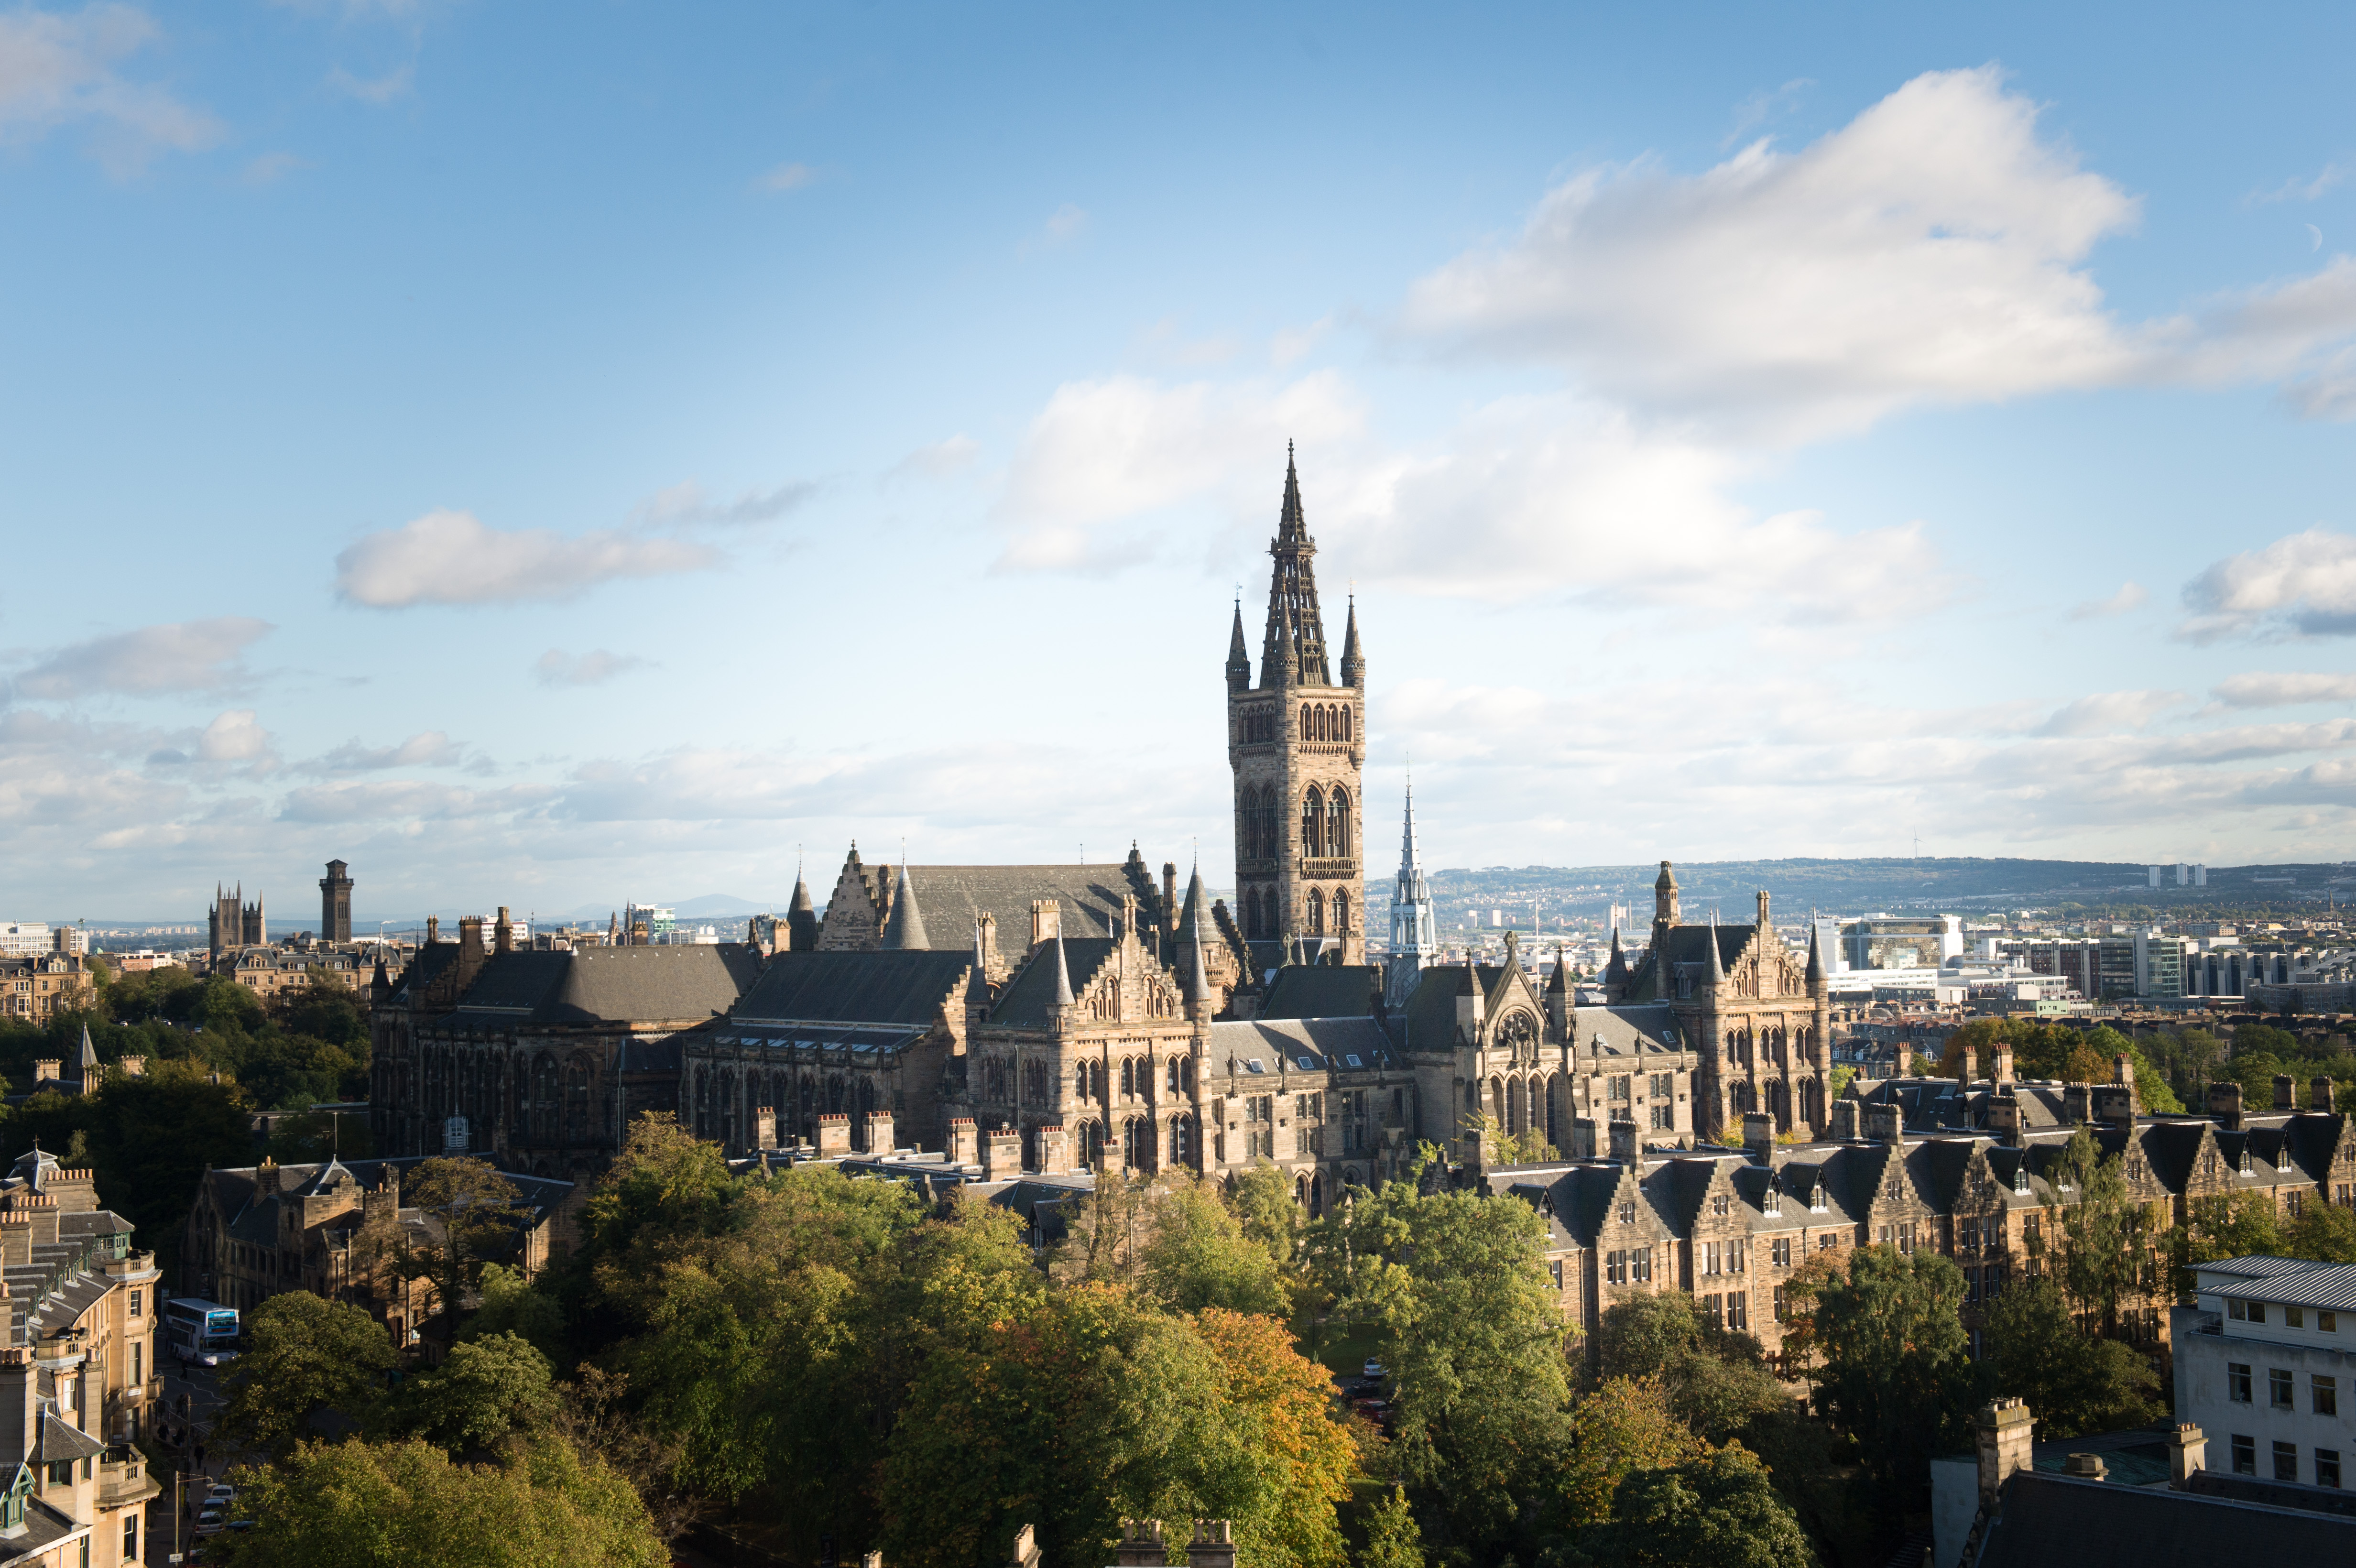
\includegraphics[keepaspectratio=true, height=\paperheight]{../../images/background.jpg}};
    }
    \begin{frame}[plain,noframenumbering]
        \titlepage
    \end{frame}
}

\section{Demotivation}

\begin{frame}{Demotivation}
    My first experience of research: a summer internship reimplementing a clique algorithm from the literature.

    \bigskip

    My code produced the ``wrong'' answer on a few instances.

    \bigskip\pause

    I spent a month trying to find and fix it.

    \bigskip\pause

    The published answers were wrong.
\end{frame}

\begin{frame}{How Do We Know Our Solvers Are Correct?}
    I've wanted to write a CP solver for years.

    \bigskip

    How will I know it's right? What if I ruin some poor student's life by publishing wrong answers?

    \bigskip\pause

    What if someone uses my solver for kidney exchange or workplace allocation or deciding adoptive parents?
\end{frame}

\begin{frame}{The Slide That Keeps Getting Me Into Trouble}
    2021 MiniZinc challenge: for 1.28\% of instances, wrong solutions were claimed.
    \\
    \begin{itemize}
        \item False claims of unsatisfiability.
        \item False claims of optimality.
        \item Infeasible solutions produced.
        \item Not limited to a single solver, problem, or constraint.
        \item Not even consistent---same solver on same hardware and same instance can give
            different results on different runs.
    \end{itemize}
    \bigskip
    I don't want my solver to produce wrong answers!

    \bigskip\pause

    Or at least, when it's wrong, I want a guaranteed way of detecting it.
\end{frame}

\begin{frame}{Proof Logging}
        \vspace*{-1em}
        \begin{center}
        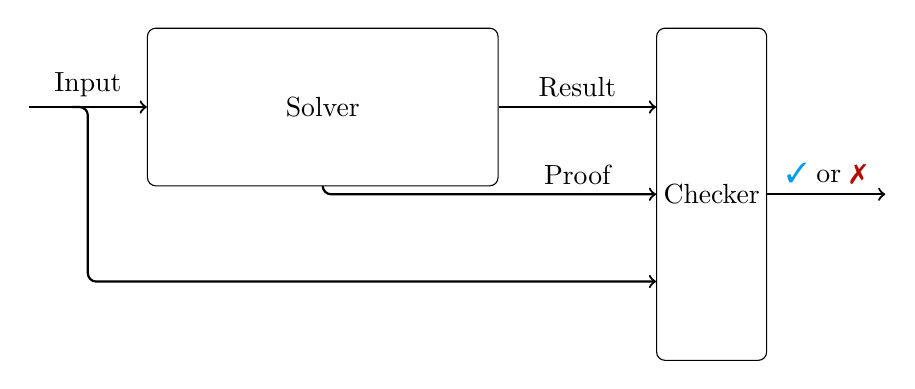
\begin{tikzpicture}
            \node (solver) [%
            inner xsep=5em,
            inner ysep=2.5em,
            draw, rounded corners=3pt] { Solver };

            \node (checker) [%
            right=2cm of solver.north east,
            anchor=north west,
            inner xsep=0.25em,
            draw, rounded corners=3pt,
            minimum height=12em,
            visible on=<3->] { Checker };

            \draw [->, thick] (solver.east) -- (solver.east -| checker.west)
                coordinate [midway] (solutionmid) node [above, midway]
                { Result };

            \draw [->, thick, rounded corners=3pt, visible on=<2->] (solver.south) -- (solver.south |- checker.west)
                -- (checker.west) coordinate [midway] (proofmid);

            \coordinate (prooflabel) at (proofmid-|solutionmid);
            \node [above=0cm of prooflabel, visible on=<2->] { Proof };

            \coordinate [right=1.5cm of checker.east] (verified);
            \draw [->, thick, visible on=<4->] (checker.east) -- (verified) node [above, midway] {
                \textcolor{uofgcobalt}{\ding{51}} or \textcolor{uofgpillarbox}{\ding{55}} };

            \coordinate [left=1.5cm of solver.west] (input);
            \draw [->, thick] (input) -- (solver.west) coordinate [midway] (inputmid) node [above, midway] { Input };

            \coordinate (checkerbotleft) at ($(checker.west)+($(checker.west)-(solver.east-|checker.west)$)$);

            \draw [->, thick, rounded corners=3pt, visible on=<3->] ($(inputmid)+(-0.2,0)$) -- (inputmid) -- (inputmid |- checkerbotleft) -- (checkerbotleft);
        \end{tikzpicture}
      \end{center}

      \vspace{-10mm}

  \begin{enumerate}
  \item<1->
    Run solver on problem input.
  \item<2->
    Get as output not only
    result   %%%   solution   % -JN
    but also proof.
  \item<3->
    Feed input +
    result   %%%   solution
    + proof to proof checker.
  \item<4->
    Verify that proof checker says
    result   %%%   solution
    is     correct.
  \end{enumerate}
\end{frame}

\section{Proof Logging for SAT}

\begin{frame}{What Is A Proof?}
    \begin{center}
        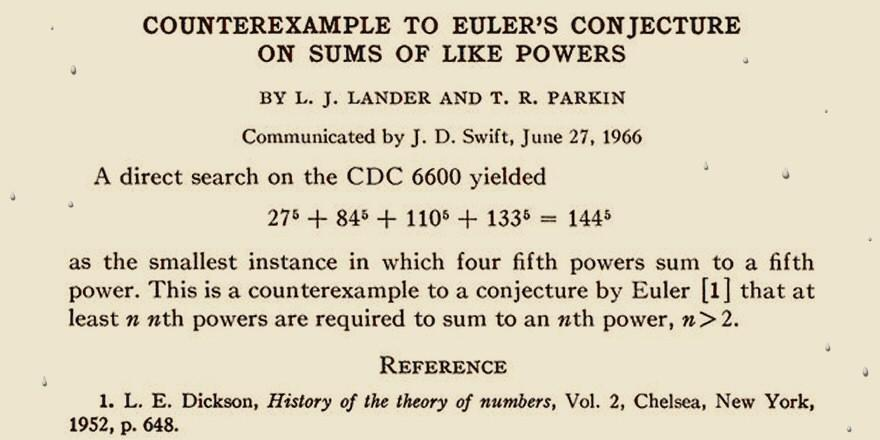
\includegraphics[keepaspectratio=true,scale=0.30]{shortest-math-paper.jpg}
    \end{center}
\end{frame}

\providecommand{\litell}{\ell}
\providecommand{\clwidth}{k}

\begin{frame}
  \frametitle{The SAT Problem}

  \vspace{-1mm}

  \begin{itemize}
  \item
      \textcolor{uofgcobalt}{Variable} $\varx$:
    takes value
%       $1$ (\textbf{true})
    \textbf{true} ($=\!1$)
    or
%       $0$ (\textbf{false})
    \textbf{false} ($=\!0$)

    \medskip

  \item
      \textcolor{uofgcobalt}{Literal}
%       $\lita$:
    $\litell$:
    variable
    $\varx$ or its negation
    $\olnot{\varx}$
%       (%which we will
%       %from now on
%       write
%       $\olnot{\varx}$
%       instead of
%       $\lnot{\varx}$)


    \medskip

  \item
      \textcolor{uofgcobalt}{Clause}
    $\clc = \litell_1 \lor \cdots \lor \litell_{\clwidth}$:
    disjunction of literals \\
    (Consider
%    clauses
    as sets, so
    no repetitions and order
%        is
    irrelevant)

    \medskip

  \item
      \textcolor{uofgcobalt}{%
      Conjunctive normal form (CNF)
%         CNF
      formula}
    $\formf = \clc_1 \land \cdots \land \clc_m$:
    conjunction of clauses

%        \bigskip
%
%      \item
%        \propfalse{\kcnfform{}}:
%        CNF formula with clauses of size $\leq \clwidth$ \\
%        (assume $\clwidth$ fixed)
%
%        \bigskip
%
%      \item
%        Refer to clauses of \cnfform as
%        \introduceterm{axioms} \\
%        (as opposed to derived clauses)
%
  \end{itemize}


%     \pause
%     \bigskip
  \medskip

  \begin{block}{The SAT Problem}
    Given a CNF formula~$\formf$, is it satisfiable?
  \end{block}

%     \pause
%     \bigskip
  \medskip

  For instance, what about:
  \begingroup
  \small
  \begin{gather*}
%       &
    ( p \lor \overline{u} )
    \land
    ( q \lor r )
    \land
    ( \overline{r} \lor w )
    \land
    ( u \lor x \lor y )
      \ \land \
    \\
%%%
%       \land \
%       &
    ( x \lor \overline{y} \lor z )
    \land
    ( \overline{x} \lor z )
    \land
    ( \overline{y} \lor \overline{z} )
    \land
    ( \overline{x} \lor \overline{z} )
    \land
    ( \overline{p} \lor \overline{u} )
  \end{gather*}
  \endgroup
%
%     For instance,
%     what about our example formula?
%     \begin{align*}
%       %        F = \ \ \ \ \
%       &
%       ( x \lor z ) \land
%       ( y \lor \olnot{z} ) \land
%       ( x \lor \olnot{y} \lor u ) \land
%       ( \olnot{y} \lor \olnot{u} ) \\
%       \land \
%       &( u \lor v ) \land
%       ( \olnot{x} \lor \olnot{v} ) \land
%       ( \olnot{u} \lor w ) \land
%       ( \olnot{x} \lor \olnot{u} \lor \olnot{w} )
%     \end{align*}
%

\end{frame}

%%% Local Variables:
%%% mode: latex
%%% TeX-master: "ProofCplxSATsurvey"
%%% End:



\begin{frame}{Proofs for SAT}

    For satisfiable instances: just
%%% THIS IS JUST confusing at this stage... -JN
%       give (something that propagates to)
    specify
    a satisfying assignment.
    \\ \medskip
    For unsatisfiability:
%       a proof is
    a sequence of clauses (CNF constraints).
    \begin{itemize}
        \item
          Each clause follows ``obviously'' from everything we know so far.
        \item
          Final clause is empty, meaning contradiction (written $\bot$).
        \item
          Means original formula must be inconsistent.
    \end{itemize}
\end{frame}

\begin{frame}[t]{What Is Obvious? Unit Propagation}


  \begin{block}{Unit Propagation}
    Clause
    $\clc$
    \colorblue{unit propagates}
    $\litell$ under partial assignment $\rho$
    if
    $\rho$ falsifies all literals in
    $\clc$ except~$\litell$.
  \end{block}

  \pause
  \bigskip

  \textbf{Example:} Unit propagate for
  $\rho = \set{ p \mapsto 0, q\mapsto 0}$ on
%
%     \vspace{-4mm}
%
  \begingroup
  \footnotesize
  \begin{equation*}%
    \cdclformulaleftadjust
    (
    \propfalse<3->{p} \lor
    \proptrue<4->{\overline{u}}
    )
    \landwsp
    ( \propfalse<3->{q}
    \lor
    \proptrue<5->{r}
    )
    \landwsp
    (
    \propfalse<5->{\overline{r}}
    \lor
    \proptrue<6->{w}
    )
    \landwsp
    (
    \propfalse<4->{u}
    \lor x \lor y )
    \landwsp
    ( x \lor \overline{y} \lor z )
    \landwsp
    ( \overline{x} \lor z )
    \landwsp
    ( \overline{y} \lor \overline{z} )
    \landwsp
    ( \overline{x} \lor \overline{z} )
    \landwsp
    (
    \proptrue<3->{\overline{p}}
    \lor
    \proptrue<4->{\overline{u}}
    )
  \end{equation*}
  \endgroup

  \vspace{-2mm}

  \begin{itemize}
  \item<4->
    $p \lor \overline{u}$ propagates $u \mapsto 0$.

  \item<5->
    $q \lor r$ propagates $r \mapsto 1$.

  \item<6->
    Then
    $\overline{r} \lor w$ propagates $w \mapsto 1$.

  \item<7->
    No further unit propagations.
  \end{itemize}

  \medskip

  \uncover<8->{%
    Proof checker should
%       be smart enough to
    know how to
    unit propagate until saturation.
  }

\end{frame}

\begin{frame}[t]%
%     {Forward Checking (DPLL)}
  {Davis-Putman-Logemann-Loveland (DPLL)}

    DPLL:
  Assign variables and propagate;
  backtrack when clause violated.

  \medskip

%%%
%%% Lots of text... Try to be more concise -JN
%%%
%     We could write a ``proof'' of unsatisfiability
%     by writing a step whenever a forward-checker backtracks
%     asserting the negation of the guesses we made. For example,
%

  ``Proof trace'':
  when backtracking, write negation
  of guesses made.


%%%%%
%%%%% Changed to an example that is simpler when highlighting is added -JN
%%%%%

  \begingroup
  \footnotesize
  \begin{equation*}%
%%%
%%% FORMULA *WITH* HIGHLIGHTING
%%%
    \cdclformulaleftadjust
    (
    \proptrue<5-5>{p}
    \lor
    \propfalse<4-5>{\overline{u}}
    )
    \landwsp
    (
    q
    \lor
    r
    )
    \landwsp
    (
    \overline{r}
    \lor
    w
    )
    \landwsp
    (
    \proptrue<4-5>{u}
    \lor
    \only<1-8>{\propfalse<2-8>{x}}
    \only<9->{\proptrue<9-10>{x}}
    \lor
    \only<1-5>{\propfalse<3-5>{y}}
    \only<6->{\proptrue<6-7>{y}}
    )
    \landwsp
    (
    \only<1-8>{\propfalse<2-8>{x}}
    \only<9->{\proptrue<9-10>{x}}
    \lor
    \only<1-5>{\proptrue<3-5>{\overline{y}}}
    \only<6->{\propfalse<6-7>{\overline{y}}}
    \lor
    \proptrue<7,10>{z}
    )
    \landwsp
    (
    \only<1-8>{\proptrue<2-8>{\overline{x}}}
    \only<9->{\propfalse<9-10>{\overline{x}}}
    \lor
    \proptrue<7,10>{z}
    )
    \landwsp
    (
    \only<1-5>{\proptrue<3-5>{\overline{y}}}
    \only<6->{\propfalse<6-7>{\overline{y}}}
    \propfalse<7>{\lor}
    \propfalse<7,10>{\overline{z}}
    )
    \landwsp
    (
    \only<1-8>{\proptrue<2-8>{\overline{x}}}
    \only<9->{\propfalse<9-10>{\overline{x}}}
    \propfalse<10>{\lor}
    \propfalse<7,10>{\overline{z}}
    )
    \landwsp
    (
    \propfalse<5-5>{\overline{p}}
    \propfalse<5-5>{\lor}
    \propfalse<4-5>{\overline{u}}
    )
%%%
%%% FORMULA WITHOUT HIGHLIGHTING
%%%
%       \cdclformulaleftadjust
%       ( p \lor \overline{u} )
%       \landwsp
%       ( q \lor r )
%       \landwsp
%       ( \overline{r} \lor w )
%       \landwsp
%       ( u \lor x \lor y )
%       \landwsp
%       ( x \lor \overline{y} \lor z )
%       \landwsp
%       ( \overline{x} \lor z )
%       \landwsp
%       ( \overline{y} \lor \overline{z} )
%       \landwsp
%       ( \overline{x} \lor \overline{z} )
%       \landwsp
%       ( \overline{p} \lor \overline{u} )
  \end{equation*}
  \endgroup

  \bigskip

  \begin{columns}[T]%
    \begin{column}{0.4\textwidth}
      \begin{enumerate}
      \item <5-> $x \lor y$
      \item <7-> $x \lor \olnot{y}$
      \item <8-> $x$
      \item <10-> $\olnot{x}$
      \item <11-> $\emptycl$
      \end{enumerate}
    \end{column}
    \begin{column}{0.5\textwidth}
%%%
%%% SEARCH TREE *WITH* OVERLAYS FOR HIGHLIGHTING
%%%
      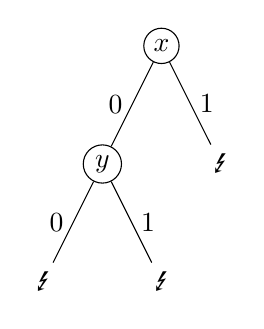
\begin{tikzpicture}<2->%
        [sibling distance=4em, level distance=3.5em, align=center]
        \node [draw, circle, inner sep=2pt, visible on=<2->] {$x$}
        child { node [draw, circle, inner sep=2pt, visible on=<3->] {$y$}
          child { node [visible on=<5->] {\Lightning} edge from parent [visible on=<3->] node [left, visible on=<3->] {
$0$  %  $\overline{y}$
} }
          child { node [visible on=<7->] {\Lightning} edge from parent [visible on=<6->] node [right, visible on=<6->] {
$1$ % $y$
} }
          edge from parent [visible on=<2->] node [left, visible on=<2->] {
$0$ % $\overline{x}$
}
        }
        child { node [visible on=<10->] {\Lightning}
          edge from parent [visible on=<9->] node [right, visible on=<9->] {
$1$  % $x$
 }
        }
        ;
      \end{tikzpicture}
    \end{column}
  \end{columns}
\end{frame}

\begin{frame}{Reverse Unit Propagation (RUP)}

  To make this a proof, need
%       each backtrack clause  %%% Trying to fit on one line -JN
  backtrack clauses
  to be easily verifiable.

  \pause

  \begin{block}{Reverse unit propagation (RUP) clause}
    $\clc$ is a
    \colorblue{reverse unit propagation (RUP)}
    clause \wrt $\formf$ if
    \begin{itemize}
    \item
      assigning $\clc$ to false,
    \item
      then unit propagating on $\formf$ until saturation
    \item
      leads to contradiction
    \end{itemize}
    If so,
    $\formf$ clearly  implies  $\clc$,
    and condition easy to verify efficiently
  \end{block}

  \pause

  \begin{block}{Fact}
%       Backtracks
    Backtrack clauses
    from DPLL solver generate a RUP proof.
  \end{block}

\end{frame}

\begin{frame}{RUP Proofs and CDCL}
\begin{block}{Fact}
  All learned clauses generated by CDCL solver are RUP clauses.
\end{block}

\pause
\bigskip

  So short proof of unsatisfiability for
  \begingroup
  \footnotesize
  \begin{equation*}%
    \cdclformulaleftadjust
    (
    \proptrue<11>{p}
    \lor
    \proptrue<3-5>{\propfalse<10-11>{\overline{u}}}
    )
    \landwsp
    {( q \lor r )}
    \landwsp
    {( \overline{r} \lor w )}
    \landwsp
    (
    \proptrue<10-11>{\propfalse<3-5>{u}}
    \lor
    \proptrue<6-7>{\propfalse<3-5,9-11>{x}}
    \lor
    \proptrue<4-5>{y}
    )
    \landwsp
    (
    \proptrue<6-7>{\propfalse<3-5,9-11>{x}}
    \lor
    \propfalse<4-5>{\overline{y}}
    \lor
    \proptrue<5,7>{z}
    )
    \landwsp
    (
    \proptrue<3-5,9-11>{\propfalse<6-7>{\overline{x}}}
    \lor
    \proptrue<5,7>{z}
    )
    \landwsp
    (
    \propfalse<4-5>{\overline{y}}
    \propfalse<5>{\lor}
    \propfalse<5,7>{\overline{z}}
    )
    \landwsp
    (
    \proptrue<3-5,9-11>{\propfalse<6-7>{\overline{x}}}
    \propfalse<7>{\lor}
    \propfalse<5,7>{\overline{z}}
    )
    \landwsp
    (
    \propfalse<11>{\overline{p}}
    \propfalse<11>{\lor}
    \proptrue<3-5>{\propfalse<10-11>{\overline{u}}}
    )
  \end{equation*}
  \endgroup
  %
  is sequence of
  reverse unit propagation (RUP)
  clauses
  \begin{enumerate}
  \item
    \propfalsenox<3-5>{$\proptrue<10-11>{u} \lor
      \proptrue<6-7>{\propfalsenox<9-11>{x}}$}
  \item
    \propfalsenox<6-7>{\proptrue<9-11>{$\olnot{x}$}}
  \item
      \propfalsenox<8-11>{$\emptycl$}
  \end{enumerate}
\end{frame}

\begin{frame}[fragile,t]{Writing Proofs in the DRAT Format}
\begingroup\footnotesize\vspace*{-3em}\begin{equation*}%
    \cdclformulaleftadjust
    (p \lor \overline{u})
    \landwsp ( q \lor r )
    \landwsp ( \overline{r} \lor w )
    \landwsp (u \lor x \lor y )
    \landwsp (x \lor \overline{y} \lor z)
    \landwsp (\overline{x} \lor z)
    \landwsp (\overline{y} \lor \overline{z})
    \landwsp (\overline{x} \lor \overline{z})
    \landwsp (\overline{p} \lor \overline{u})
\end{equation*}\endgroup\vspace*{-1em}%
\begin{columns}[t]
        \column{0.33\textwidth}\begin{onlyenv}<2->%  Avoid spurious blank -JN
        \colorblue{In DIMACS} \\
\begin{Verbatim}
p cnf 8 9
1 -4 0
2 3 0
-2 5 0
4 6 7 0
6 -7 8 0
-6 8 0
-7 -8 0
-6 -8 0
-1 -4 0
\end{Verbatim}
\end{onlyenv}\column{0.33\textwidth}\begin{onlyenv}<3->%
\colorblue{DPLL Proof
%     (RUP)
  in RUP
}
      $x \lor y$ \\
      $x \lor \olnot{y}$ \\
      $x$ \\
      $\olnot{x}$ \\
      $\emptycl$ \\
      \medskip

\end{onlyenv}\begin{onlyenv}<4->\colorblue{DPLL Proof in DRAT}
\begin{Verbatim}
6 7 0
6 -7 0
6 0
-6 0
0
\end{Verbatim}
\end{onlyenv}\column{0.33\textwidth}%
\begin{onlyenv}<5->\colorblue{CDCL Proof
%       (RUP)
    in RUP
  }\\
        $u \lor \varx$ \\
        $\olnot{x}$ \\
        $\emptycl$ \\
        \medskip
\end{onlyenv}
\vspace*{9.6mm}
\begin{overprint}\onslide<6->\colorblue{CDCL Proof in DRAT}
\begin{Verbatim}
4 6 0
-6 0
0
\end{Verbatim}
\end{overprint}\end{columns}
\end{frame}

\begin{frame}{Resolution Proofs}
    \begin{block}{Fact}
        RUP proofs can be seen as shorthand for Resolution proofs.
    \end{block}

    \bigskip

    \begin{minipage}[c]{0.25\framewidth}
        \textcolor{uofgcobalt}{\textbf{Model axioms}}
    \end{minipage}\hfill\begin{minipage}[c]{0.70\framewidth}
        \centering From the input
    \end{minipage}\bigskip

    \begin{minipage}[c]{0.25\framewidth}
        \textcolor{uofgcobalt}{\textbf{Resolution}}
    \end{minipage}\hfill\begin{minipage}[c]{0.70\framewidth}\begin{prooftree}
        \AxiomC{$\textcolor{uofglawn}{x_1} \vee \textcolor{uofglawn}{x_2} \vee \ldots \vee
        \textcolor{uofglawn}{x_i} \vee \textcolor{uofgpillarbox}{c}$}
        \AxiomC{$\textcolor{uofgpillarbox}{\overline{c}} \vee \textcolor{uofgcobalt}{y_1} \vee
        \textcolor{uofgcobalt}{y_2} \vee \ldots \textcolor{uofgcobalt}{y_j}$}
        \BinaryInfC{$\textcolor{uofglawn}{x_1} \vee \textcolor{uofglawn}{x_2} \vee \ldots \vee
        \textcolor{uofglawn}{x_i} \vee \textcolor{uofgcobalt}{y_1} \vee
        \textcolor{uofgcobalt}{y_2} \vee \ldots \vee \textcolor{uofgcobalt}{y_j}$}
    \end{prooftree}\end{minipage}

    \bigskip

    \begin{itemize}
        \item To prove unsatisfiability: resolve until you reach the empty clause.
    \end{itemize}
\end{frame}

\begin{frame}{Reusing DRAT Isn't Feasible}
    \begin{itemize}
        \item Stronger reasoning is hard in theory and in practice.
            \begin{itemize}
                \item Resolution can't count efficiently.
            \end{itemize}
        \item Closely tied to how MiniSAT works:
            \begin{itemize}
                \item Proofs are (mostly) sequences of learned clauses.
                \item Something special and strange happens to learned unit clauses.
            \end{itemize}
        \item Preprocessing is possible (sometimes), but not easy.
            \begin{itemize}
                \item We need to do full-on reformulation, though.
            \end{itemize}
        \item Not clear how to do optimisation, enumeration, counting, \ldots
    \end{itemize}
\end{frame}

\begin{frame}{Opinionated Requirements For This To Work}
    \begin{enumerate}
        \item Efficiently work with what solvers actually do, not idealised algorithms. \pause
        \item No need for a new proof format for every new propagator or solver.
            \begin{itemize}
                \item Constraint programming has 423 different global constraints, many of which
                    have several different propagators.
                \item Some propagators are buggy, and at least one has faulty theory behind it\ldots
            \end{itemize} \pause
        \item Proof format must still be simple and well-founded.
            \begin{itemize}
                \item Need to be able to trust the verifier.
                \item Interactions between features can be subtle: even deletions aren't that easy
                    to get right.
            \end{itemize}
    \end{enumerate}
\end{frame}

\begin{frame}[fragile]{Unexpected and Remarkable Claim}
    \begin{itemize}
        \item We can do everything we want with a proof format which is only slightly more
            sophisticated than DRAT.
        \item <2-> Using proof logs during development leads to faster development than not doing proof logging.
        \item <3-> You should make your students and postdocs adopt this technology right now.
    \end{itemize}
\end{frame}

\section{Beyond SAT}

\begin{frame}{From CNF to Pseudo-Boolean}
    \begin{itemize}
        \item A set of $\{ 0, 1 \}$-valued variables $x_i$, $1$ means true.
        \item Constraints are linear inequalities \[
                \sum_i c_i x_i \ge C
            \]
        \item Write $\overline{x}_i$ to mean $1 - x_i$.
        \item Can rewrite CNF to pseudo-Boolean directly, \begin{align*}
                & x_1 \vee \overline{x}_2 \vee x_3 & \leftrightarrow && x_1 + \overline{x}_2 + x_3 \ge 1
        \end{align*}
    \end{itemize}
\end{frame}

\begin{frame}{Cutting Planes Proofs}
    \begin{minipage}[c]{0.35\framewidth}
        \textcolor{uofgcobalt}{\textbf{Model axioms}}
    \end{minipage}\hfill\begin{minipage}[c]{0.60\framewidth}
        \centering From the input
    \end{minipage}\bigskip

    \begin{minipage}[c]{0.35\framewidth}
        \textcolor{uofgcobalt}{\textbf{Literal axioms}}
    \end{minipage}\hfill\begin{minipage}[c]{0.60\framewidth}\begin{prooftree}
        \AxiomC{~}
        \UnaryInfC{$\ell_i \ge 0$}
    \end{prooftree}\end{minipage}\bigskip

    \begin{minipage}[c]{0.35\framewidth}
        \textcolor{uofgcobalt}{\textbf{Addition}}
    \end{minipage}\hfill\begin{minipage}[c]{0.60\framewidth}\begin{prooftree}
        \AxiomC{$\sum_i a_i \ell_i \ge A$}
        \AxiomC{$\sum_i b_i \ell_i \ge B$}
        \BinaryInfC{$\sum_i (a_i + b_i) \ell_i \ge A + B$}
    \end{prooftree}\end{minipage}\bigskip

    \begin{minipage}[c]{0.35\framewidth}
        \textcolor{uofgcobalt}{\textbf{Multiplication}}\\
        for any $c \in \mathbb{N^+}$
    \end{minipage}\hfill\begin{minipage}[c]{0.60\framewidth}\begin{prooftree}
        \AxiomC{$\sum_i a_i \ell_i \ge A$}
        \UnaryInfC{$\sum_i { c a_i \ell_i } \ge c A$}
    \end{prooftree}\end{minipage}\bigskip

    \begin{minipage}[c]{0.35\framewidth}
        \textcolor{uofgcobalt}{\textbf{Division}}\\
        for any $c \in \mathbb{N^+}$
    \end{minipage}\hfill\begin{minipage}[c]{0.60\framewidth}\begin{prooftree}
        \AxiomC{$\sum_i a_i \ell_i \ge A$}
        \UnaryInfC{$\sum_i {\left\lceil \frac{a_i}{c} \right\rceil} \ell_i \ge \left\lceil \frac{A}{c} \right\rceil$}
    \end{prooftree}\end{minipage}\bigskip
\end{frame}

\begin{frame}{Extension Variables}
  Suppose we want new, fresh variable
  $a$ encoding
  \begin{equation*}
      \textcolor{uofglawn}{
        a
        \lequiv
        ( 3x + 2y + z + w \ge 3 )
%           (\varx \land y)
      }
  \end{equation*}

  Introduce constraints
  \begin{equation*}
      \textcolor{uofgcobalt}{
%           a \lor \olnot{\varx} \lor \olnot{y}
%       \qquad
    3 \olnot{a} + 3x + 2y + z + w \ge 3
%       \olnot{a} \lor \varx
    \qquad
    5 a +
    3 \olnot{x} + 2 \olnot{y}  + \olnot{z} + \olnot{w} \ge 5
%       \olnot{a} \lor y
}
  \end{equation*}

  Should be fine, so long as $a$ hasn't been used before.
\end{frame}

\begin{frame}{Interleaving RUP and Extended Cutting Planes}
    \begin{itemize}
        \item Can define RUP similarly for pseudo-Boolean constraints.
            \begin{itemize}
            \item It does the same thing on clauses.
            \item Should probably be called ``reverse integer bounds consistency''.
            \end{itemize}
        \item Idea: use RUP for backtracking, and include explicit extended cutting
            planes steps to justify reasoning.
    \end{itemize}
\end{frame}

\begin{frame}{Proof Logs for Extended Cutting Planes}
    For satisfiable instances: just specify a satisfying assignment.
    \\ \medskip
    For unsatisfiability: a sequence of
    \colorblue{pseudo-Boolean constraints}.
    \begin{itemize}
        \item Each constraint follows ``obviously'' from what is known
          so far.
        \item Either implicitly, by RUP\ldots
        \item Or by
          an explicit cutting planes derivation\ldots
        \item Or as an extension variable reifying a new constraint
        \item Final constraint is $0 \ge 1$.
    \end{itemize}
\end{frame}

\begin{frame}{Enumeration and Optimisation Problems}

  Enumeration:
  \begin{itemize}
  \item
    When a solution is found, can log it.
  \item Introduces a new constraint saying ``not this solution''.
  \item So the proof semantics are ``unsatisfiable, except for all the solutions I told you about''.
  \end{itemize}

  \medskip
  \pause

  For optimisation:
  \begin{itemize}
  \item Define an objective
      \textcolor{uofgcobalt}{$f = \sum_i w_i \ell_i$},
    $w_i \in \mathbb{Z}$,
    to minimise in the pseudo-Boolean model.
  \item
    To maximise, negate objective.
  \item Log a solution
    $\alpha$,
    get a solution-improving constraint
          \textcolor{uofgcobalt}{$\sum_i w_i \ell_i \leq -1 + \sum_i w_i \alpha(\ell_i)$}.
  \end{itemize}
\end{frame}

\begin{frame}{The VeriPB System}
    \begin{center}
        \url{https://gitlab.com/MIAOresearch/software/VeriPB} \\
        \bigskip
    \end{center}
    \begin{itemize}
        \item MIT licence, written in Python with parsing in C++.
        \item Useful features like tracing and proof debugging.
    \end{itemize}
\end{frame}

\section{Proof Logging for CP}

\begin{frame}{Making a Proof-Logging Solver}
    \begin{enumerate}
        \item Output a pseudo-Boolean encoding of the problem.
        \item Make the solver log its search tree.
            \begin{itemize}
                \item Output a small header.
                \item Output something on every backtrack.
                \item Output something every time a solution is found.
                \item Output a small footer.
            \end{itemize}
        \item Figure out how to log propagations.
    \end{enumerate}
\end{frame}

\begin{frame}{A Slightly Different Workflow}
    \begin{center}
        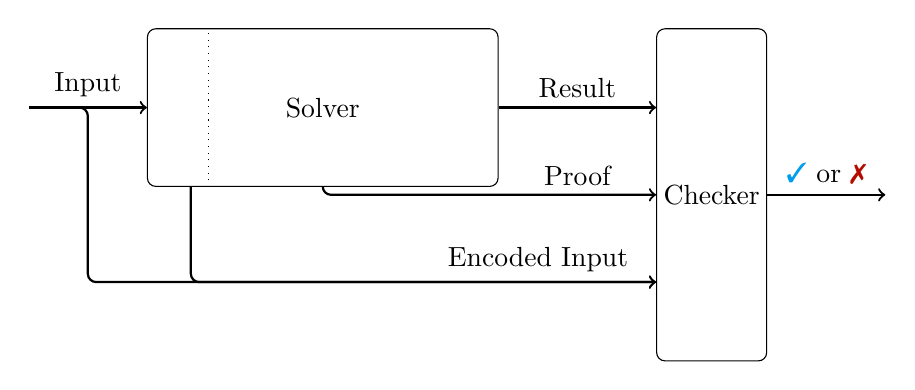
\begin{tikzpicture}
            \node (solver) [inner xsep=5em, inner ysep=2.5em, draw, rounded corners=3pt] { Solver };

            \node (checker) [right=2cm of solver.north east, anchor=north west,
            inner xsep=0.25em, draw, rounded corners=3pt, minimum height=12em, visible on=<3->] { Checker };

            \draw [->, thick] (solver.east) -- (solver.east -| checker.west)
                coordinate [midway] (solutionmid) node [above, midway] { Result };

            \draw [->, thick, rounded corners=3pt, visible on=<2->] (solver.south) -- (solver.south |- checker.west)
                -- (checker.west) coordinate [midway] (proofmid);

            \coordinate (prooflabel) at (proofmid-|solutionmid);
            \node [above=0cm of prooflabel, visible on=<2->] { Proof };

            \coordinate [right=1.5cm of checker.east] (verified);
            \draw [->, thick, visible on=<5->] (checker.east) -- (verified) node [above, midway] {
                \textcolor{uofgcobalt}{\ding{51}} or \colorred{\ding{55}} };

            \coordinate [left=1.5cm of solver.west] (input);
            \draw [->, thick] (input) -- (solver.west) coordinate [midway] (inputmid) node [above, midway] { Input };

            \coordinate (checkerbotleft) at ($(checker.west)+($(checker.west)-(solver.east-|checker.west)$)$);

            \draw [->, thick, rounded corners=3pt, visible on=<3>] ($(inputmid)+(-0.2,0)$) --
            (inputmid) -- (inputmid |- checkerbotleft) -- (checkerbotleft) coordinate [midway] (altinputmid);
            \coordinate (solverstart) at ($(solver.south)!0.75!(solver.south west)$);
            \coordinate (solverstart2) at ($(solver.south)!0.65!(solver.south west)$);
            \draw [dotted, visible on=<4->] (solverstart2) -- (solverstart2 |- solver.north);
            \draw [->, thick, rounded corners=3pt, visible on=<4->] (solverstart) -- (solverstart |- checkerbotleft) -- (checkerbotleft);

            \coordinate (prooflabel) at (altinputmid-|solutionmid);
            \node [above=0cm of prooflabel, xshift=-0.5cm, visible on=<4->] { Encoded Input };
        \end{tikzpicture}
    \end{center}
\end{frame}

\begin{frame}[t]{Compiling CP Variables}
    Given $A \in \{ -3 \ldots 9 \}$:
\only<1>{
    \begin{align*}
        a_{{=}-3} + a_{{=}-2} + a_{{=}-1} + a_{{=}0} + a_{{=}1} + a_{{=}2}
        + a_{{=}3} \\ +~a_{{=}4} + a_{{=}5} + a_{{=}6} + a_{{=}7}
        + a_{{=}8} + a_{{=}9} &= 1
    \end{align*}
}\only<2->{
\begin{align*}
    -32 a_{{\operatorname{neg}}} + 1 a_{{\operatorname{b}}0} + 2 a_{{\operatorname{b}}1} + 4
    a_{{\operatorname{b}}2} + 8 a_{{\operatorname{b}}3} + 16 a_{{\operatorname{b}}4} &\ge -3
    \textnormal{~and}\\
    32 a_{{\operatorname{neg}}} + -1 a_{{\operatorname{b}}0} + -2 a_{{\operatorname{b}}1} +
    -4 a_{{\operatorname{b}}2} + -8 a_{{\operatorname{b}}3} + -16 a_{{\operatorname{b}}4} &\ge -9
\end{align*}

    \only<3->{
    Then where needed, define:
    \begin{align*}
        a_{{\ge}4} & \leftrightarrow -32 a_{{\operatorname{neg}}} + 1 a_{{\operatorname{b}}0} + 2 a_{{\operatorname{b}}1} + 4
        a_{{\operatorname{b}}2} + 8 a_{{\operatorname{b}}3} + 16 a_{{\operatorname{b}}4} &\ge 4 \\
        a_{{\ge}5} & \leftrightarrow -32 a_{{\operatorname{neg}}} + 1 a_{{\operatorname{b}}0} + 2 a_{{\operatorname{b}}1} + 4
        a_{{\operatorname{b}}2} + 8 a_{{\operatorname{b}}3} + 16 a_{{\operatorname{b}}4} &\ge 5 \\
        a_{{=}4} & \leftrightarrow a_{{\ge}4} \land \overline{a}_{{\ge}5}
    \end{align*}

    We can do this in the pseudo-Boolean model, where needed, or lazily inside
    the proof using extension variables.
}}
\end{frame}

\begin{frame}{Introducing Useful Facts About Variables}
    When creating $x_{{=}i}$, also introduce
    \begin{align*}
        x_{{\ge}i} \rightarrow x_{{\ge}j} \quad \text{and} \quad x_{{\ge}h} \rightarrow x_{{\ge}i}
    \end{align*}
    for the closest two values $h$ and $j$ that already have equality variables.

    \bigskip\pause

    All-different is easier if we introduce \begin{align*}
    \sum_{i=\ell}^{u} x_{{=}i} \ge 1
    \end{align*}
    which is also easy to do in a proof.
\end{frame}

\begin{frame}{Compiling Constraints}
    \only<1>{
        \begin{itemize}
            \item Also need to compile every constraint to pseudo-Boolean form.
            \item Doesn't need to be a propagating encoding.
            \item Can use additional variables.
        \end{itemize}
    }\only<2>{
    Given $2A + 3B + 4C \ge 42$, where $A, B, C \in \{ -3 \ldots 9 \}$,
\begin{align*}
    -64 a_{{\operatorname{neg}}} + 2 a_{{\operatorname{b}}0} + 4 a_{{\operatorname{b}}1} + 8
    a_{{\operatorname{b}}2} + 16 a_{{\operatorname{b}}3} + 32 a_{{\operatorname{b}}4} \\
    + -96 b_{{\operatorname{neg}}} + 3 b_{{\operatorname{b}}0} + 6
    b_{{\operatorname{b}}1} + 12 b_{{\operatorname{b}}2} + 24 b_{{\operatorname{b}}3} + 48
    b_{{\operatorname{b}}4} \\
    + -128 c_{{\operatorname{neg}}} + 4 c_{{\operatorname{b}}0} + 8
    c_{{\operatorname{b}}1} + 16 c_{{\operatorname{b}}2} + 32 c_{{\operatorname{b}}3} + 64
    c_{{\operatorname{b}}4} & \ge 42 \textnormal{.}
\end{align*}}\only<3>{
    Given $(A, B, C) \in [(1, 2, 3), (1, 3, 4), (2, 2, 5)]$, define
    \begin{align*}
        3\overline{t}_{0} + a_{{=}1} + b_{{=}2} + c_{{=}3} \ge 3 &\quad \text{i.e.}&t_{0} \rightarrow (a_{{=}1} \wedge b_{{=}2} \wedge c_{{=}3}) \\
        3\overline{t}_{1} + a_{{=}1} + b_{{=}4} + c_{{=}4} \ge 3 &\quad \text{i.e.}&t_{1} \rightarrow (a_{{=}1} \wedge b_{{=}4} \wedge c_{{=}4}) \\
        3\overline{t}_{2} + a_{{=}2} + b_{{=}2} + c_{{=}5} \ge 3 &\quad \text{i.e.}&t_{2} \rightarrow (a_{{=}2} \wedge b_{{=}2} \wedge c_{{=}5})
    \end{align*} using a tuple selector variable \begin{align*}
        &t_{0} + t_{1} + t_{2} = 1
    \end{align*}}
\end{frame}

\begin{frame}{Proof Logging Search Trees}
    Want to just output a reverse unit propagation step on every backtrack.

    \bigskip

    This works for forward-checking / DPLL, but not with strong propagators.

    \bigskip

    The key invariant: any propagation visible to the CP solver must be reflected either
    \begin{itemize}
        \item By ``unit propagation'' on the pseudo-Boolean model,
        \item Or by reverse unit propagation on the backtrack clause.
    \end{itemize}
\end{frame}

\begin{frame}{Proof Logging Inference: The Easy Cases}
    If it follows from bounds consistency on the pseudo-Boolean model,
    no further proof logging needed.

    \bigskip

    For example, a tuple in a table constraint becoming infeasible.

    \bigskip

    Intuition: some facts are so obvious they don't need stated.
\end{frame}

\begin{frame}{Proof Logging Inference: Using RUP}
    Some facts are ``obvious'' once we tell the proof verifier they are true,
    but not otherwise.

    \bigskip

    For example, a variable losing a value due to a table constraint.

    \bigskip

    We log these propagations using RUP.

    \bigskip

    Intuition: like singleton arc consistency.
\end{frame}

\begin{frame}{Proof Logging Inference: Explicit Justifications}
    Some facts aren't ``obvious'' but can be justified explicitly.

    \bigskip

    All-different: sum up the ``variable takes at least one value'' and ``value is used at most
    once'' constraints for a Hall set or Hall violator.

    \bigskip

    Integer linear inequalities: the slack algorithm gives an easy proof.
\end{frame}

\begin{frame}[t]{Justifying All-Different Failures}
    \begin{tabular}{r@{\hspace*{0mm}}c@{\hspace*{0.6mm}}c@{\hspace*{0.6mm}}c@{\hspace{0.6mm}}c@{\hspace*{0.6mm}}r@{\hspace*{3mm}}r@{\hspace*{0.8mm}}r@{\hspace*{0.8mm}}r@{\hspace*{0.8mm}}r@{\hspace*{0.8mm}}r@{\hspace*{0.8mm}}r@{\hspace*{0.8mm}}r@{\hspace*{0.8mm}}r@{\hspace*{0.8mm}}r@{\hspace*{0.8mm}}l}
    $V \in \{$ &
    1 &
      &
      &
        4 \hspace*{1.2mm} 5 &
    $\}$ & \phantom{$-v_{{=}1}$}
        &
        & \phantom{$-w_{{=}1}$}
        &
        & \phantom{$-x_{{=}1}$}
    &
        & \phantom{$-y_{{=}1}$}
    &
        & \phantom{$-z_{{=}1}$}
    &
    \\

        $\only<1>{W}\only<2->{{\color{uofgcobalt}W}} \in \{$ &
    1 &
    2 &
    3 &
        &
    $\}$ &
        $\only<1-2>{\phantom{w_{{=}1}}}\only<3->{w_{{=}1}}$ &
        $\only<1-2>{\phantom{+}}\only<3->{+}$ &
        $\only<1-2>{\phantom{w_{{=}2}}}\only<3->{w_{{=}2}}$ &
        $\only<1-2>{\phantom{+}}\only<3->{+}$ &
        $\only<1-2>{\phantom{w_{{=}3}}}\only<3->{w_{{=}3}}$ &
    &
    &
        &
        &
        $\only<1-2>{\phantom{ \ge 1}}\only<3->{ \ge 1}$
        \\

        $\only<1>{X}\only<2->{{\color{uofgcobalt}X}} \in \{$ &
    &
    2 &
    3 &
        &
    $\}$ &
        &
        &
        $\only<1-3>{\phantom{x_{{=}2}}}\only<4->{x_{{=}2}}$ &
        $\only<1-3>{\phantom{+}}\only<4->{+}$ &
        $\only<1-3>{\phantom{x_{{=}3}}}\only<4->{x_{{=}3}}$ &
        &
        &
        &
        &
        $\only<1-3>{\phantom{ \ge 1}}\only<4->{ \ge 1}$
        \\

        $\only<1>{Y}\only<2->{{\color{uofgcobalt}Y}} \in \{$ &
    1 &
    &
    3 &
        &
    $\}$ &
        $\only<1-3>{\phantom{y_{{=}1}}}\only<4->{y_{{=}1}}$ &
        &
        &
        $\only<1-3>{\phantom{+}}\only<4->{+}$ &
        $\only<1-3>{\phantom{y_{{=}3}}}\only<4->{y_{{=}3}}$ &
    &
    &
        &
        &
        $\only<1-3>{\phantom{ \ge 1}}\only<4->{ \ge 1}$
        \\

        $\only<1>{Z}\only<2->{{\color{uofgcobalt}Z}} \in \{$ &
    1 &
    &
    3 &
        &
    $\}$ &
        $\only<1-3>{\phantom{z_{{=}1}}}\only<4->{z_{{=}1}}$ &
        &
        &
        $\only<1-3>{\phantom{+}}\only<4->{+}$ &
        $\only<1-3>{\phantom{z_{{=}3}}}\only<4->{z_{{=}3}}$ &
    &
    &
        &
        &
        $\only<1-3>{\phantom{ \ge 1}}\only<4->{ \ge 1}$
        \\[0.5cm]

        \only<5->{
    &
    $\rightarrow$ &
    &
    &
    &
    &
    $-v_{{=}1}$ &
    $+$ &
    $-w_{{=}1}$ &
    $+$ &
    &
     &
    $-y_{{=}1}$ &
    $+$ &
    $-z_{{=}1}$ &
    $ \ge -1$ \\

    &
    &
    $\rightarrow$ &
    &
    &
    &
    &
    &
    $-w_{{=}2}$ &
    $+$ &
    $-x_{{=}2}$ &
     &
    &
     &
    &
    $ \ge -1$ \\

    &
    &
    &
    $\rightarrow$ &
    &
    &
    &
    &
    $-w_{{=}3}$ &
    $+$ &
    $-x_{{=}3}$ &
    $+$ &
    $-y_{{=}3}$ &
    $+$ &
    $-z_{{=}3}$ &
    $ \ge -1$
    \\[0.5cm]
}
\only<6->{
    &
    &
    &
    &
    &
    &
    $-v_{{=}1}$ &
     &
    &
    &
    &
     &
     &
     &
     &
    $ \ge 1$ \\
}
\only<7->{
    &
    &
    &
    &
    &
    &
    $ v_{{=}1}$ &
     &
    &
    &
    &
     &
     &
     &
     &
    $ \ge 0$ \\[0.5cm]
}
\only<8->{
    &
    &
    &
    &
    &
    &
    $0$ &
     &
    &
    &
    &
     &
     &
     &
     &
    $ \ge 1$ \\
}
    &
    $\phantom{\rightarrow}$ &
    $\phantom{\rightarrow}$ &
    $\phantom{\rightarrow}$ &
    &
    &
    $\phantom{-v_{{=}1}}$ &
    $\phantom{+}$ &
    $\phantom{-w_{{=}1}}$ &
    $\phantom{+}$ &
    $\phantom{-y_{{=}1}}$ &
    $\phantom{+}$ &
    $\phantom{-y_{{=}1}}$ &
    $\phantom{+}$ &
    $\phantom{-z_{{=}1}}$ &
    $\phantom{ \ge -1}$ \\
    \end{tabular}
\end{frame}

\begin{frame}{Proof Logging Reformulations}
    Some reformulations can be done inside the proof log:

    \begin{itemize}
        \item Turning not-equals from sums into binary constraints.
        \item 2D element constraints.
        \item Autotabulation.
    \end{itemize}
\end{frame}

\begin{frame}[t]{Symmetry Elimination}
    \begin{columns}[t]
    \column{0.51\textwidth}\uncover<2->{Human modellers might add:
    \begin{itemize}
    \item $A < G$ (mirror vertically)
    \item $A < B$ (mirror horizontally)
    \item $A \leq 4$ (value symmetry)
    \end{itemize}

    \smallskip

        \uncover<3->{Are these valid simultaneously?}
}%
    \column{0.45\textwidth}
    \vspace{-1.8cm}
        \onslide<1->
        \begin{block}{The Crystal Maze Puzzle}\begin{center}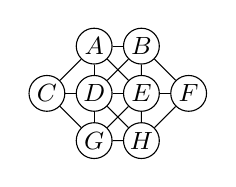
\begin{tikzpicture}[scale=0.6]
        \node [draw, circle, inner sep=1pt] (A) at (0, 0) { \phantom{X} }; \node at (A) { \small $A$ };
        \node [draw, circle, inner sep=1pt] (B) at (1, 0) { \phantom{X} }; \node at (B) { \small $B$ };
        \node [draw, circle, inner sep=1pt] (C) at (-1, -1) { \phantom{X} }; \node at (C) { \small $C$ };
        \node [draw, circle, inner sep=1pt] (D) at (0, -1) { \phantom{X} }; \node at (D) { \small $D$ };
        \node [draw, circle, inner sep=1pt] (E) at (1, -1) { \phantom{X} }; \node at (E) { \small $E$ };
        \node [draw, circle, inner sep=1pt] (F) at (2, -1) { \phantom{X} }; \node at (F) { \small $F$ };
        \node [draw, circle, inner sep=1pt] (G) at (0, -2) { \phantom{X} }; \node at (G) { \small $G$ };
        \node [draw, circle, inner sep=1pt] (H) at (1, -2) { \phantom{X} }; \node at (H) { \small $H$ };
        \draw (A) -- (B);
        \draw (A) -- (C);
        \draw (A) -- (D);
        \draw (A) -- (E);
        \draw (B) -- (D);
        \draw (B) -- (E);
        \draw (B) -- (F);
        \draw (C) -- (D);
        \draw (C) -- (G);
        \draw (D) -- (E);
        \draw (D) -- (G);
        \draw (D) -- (H);
        \draw (E) -- (F);
        \draw (E) -- (G);
        \draw (E) -- (H);
        \draw (F) -- (H);
        \draw (G) -- (H);
    \end{tikzpicture}\end{center}
    \vspace{-0.1cm}\small
    Place numbers 1 to 8 without repetition, adjacent circles cannot have
        consecutive numbers.\end{block}

    \end{columns}\medskip

  \uncover<4->{%
      We can introduce these constraints \textcolor{uofgcobalt}{inside the proof}, rather than as part of the
        pseudo-Boolean model. Based upon a \emph{dominance} rule, no group theory required!}
\end{frame}

\begin{frame}{The Glasgow Constraint Solver}
    \begin{center}
        \raisebox{-0.3em}{\url{https://github.com/ciaranm/glasgow-constraint-solver}}
        \bigskip
    \end{center}
    \begin{itemize}
        \item MIT licence, written in fancy modern C++.
        \item A growing collection of global constraints:
            \begin{itemize}
                \item Absolute value.
                \item All-different.
                \item Circuit (check and prevent).
                \item Element.
                \item Integer linear (in)equalities (with large domains, and GAC
                    reformulation).
                \item Minumum and Maximum.
                \item Regular (and hence Stretch, Geost, DiffN).
                \item Smart Table (and hence Lex, At Most One, Not All Equal).
            \end{itemize}
        \item I couldn't think of a name.
    \end{itemize}
\end{frame}

\begin{frame}[fragile,t]{A VeriPB Proof for a CP Problem}%
\vspace*{-1.5em}\begin{columns}[t]%
\column{0.25\textwidth}\small%
\begin{align*}
    &A \in \{1\ldots 5\} \\
    &B \in \{1\ldots 2\} \\
    &C \in \{2\ldots 3\} \\
    &D \in \{2\ldots 3\} \\
    &\operatorname{AllDiff}(A, B, C, D) \\
    &A + B + C \le 9 \\
    &\operatorname{minimise} 2A + 3D
\end{align*}
\column{0.7\textwidth}%
\begin{onlyenv}<1>\tiny%
\begin{Verbatim}
Problem p;
auto va = p.create_integer_variable(1_i, 5_i, "a");
auto vb = p.create_integer_variable(1_i, 2_i, "b");
auto vc = p.create_integer_variable(2_i, 3_i, "c");
auto vd = p.create_integer_variable(2_i, 3_i, "d");
p.post(AllDifferent({va, vb, vc, vd}));
p.post(LinearLessEqual{Linear{{1_i, va}, {1_i, vb}, {1_i, vc}}, 9_i});

auto obj = p.create_integer_variable(0_i, 10000_i, "obj");
p.post(LinearEquality{Linear{{2_i, va}, {3_i, vd}, {-1_i, obj}}, 0_i});
p.minimise(obj);

cout << solve_with(p,
    SolveCallbacks{
        .solution = [&](const CurrentState & s) -> bool {
            cout << "a = " << s(va) << " b = " << s(vb) << " c = " << s(vc)
                << " d = " << s(vd) << " obj = " << s(obj) << endl;
            return true;
        },
    },
    ProofOptions{"tutorial.opb", "tutorial.veripb"});
\end{Verbatim}
\end{onlyenv}\begin{onlyenv}<2>%
\begin{Verbatim}
$ ./build/tutorial_proof
a = 4 b = 1 c = 2 d = 3 obj = 17
a = 4 b = 1 c = 3 d = 2 obj = 14
propagators: 3
recursions: 5
failures: 1
propagations: 20 7 0
max depth:  2
solutions: 2
solve time: 0.001696s
\end{Verbatim}
\end{onlyenv}\begin{onlyenv}<3>\tiny%
\begin{Verbatim}
* #variable= 38 #constraint= 48
min: 1 xObj_b_0 2 xObj_b_1 4 xObj_b_2 8 xObj_b_3 16 xObj_b_4 32 xObj_b_5
    64 xObj_b_6 128 xObj_b_7 256 xObj_b_8 512 xObj_b_9 1024 xObj_b_10
    2048 xObj_b_11 4096 xObj_b_12 8192 xObj_b_13 ;
* variable xA_a 1 .. 5 bits encoding
1 xA_b_0 2 xA_b_1 4 xA_b_2 >= 1 ;
-1 xA_b_0 -2 xA_b_1 -4 xA_b_2 >= -5 ;
* variable xB_b 1 .. 2 bits encoding
1 xB_b_0 2 xB_b_1 >= 1 ;
-1 xB_b_0 -2 xB_b_1 >= -2 ;
* variable xC_c 2 .. 3 bits encoding
1 xC_b_0 2 xC_b_1 >= 2 ;
-1 xC_b_0 -2 xC_b_1 >= -3 ;
* variable xD_d 2 .. 3 bits encoding
1 xD_b_0 2 xD_b_1 >= 2 ;
-1 xD_b_0 -2 xD_b_1 >= -3 ;
* variable xObj_obj 0 .. 10000 bits encoding
1 xObj_b_0 2 xObj_b_1 4 xObj_b_2 8 xObj_b_3 16 xObj_b_4 32 xObj_b_5
    64 xObj_b_6 128 xObj_b_7 256 xObj_b_8 512 xObj_b_9 1024 xObj_b_10
    2048 xObj_b_11 4096 xObj_b_12 8192 xObj_b_13 >= 0 ;
-1 xObj_b_0 -2 xObj_b_1 -4 xObj_b_2 -8 xObj_b_3 -16 xObj_b_4 -32 xObj_b_5
    -64 xObj_b_6 -128 xObj_b_7 -256 xObj_b_8 -512 xObj_b_9 -1024 xObj_b_10
    -2048 xObj_b_11 -4096 xObj_b_12 -8192 xObj_b_13 >= -10000 ;
\end{Verbatim}
\end{onlyenv}\begin{onlyenv}<4>\tiny%
\begin{Verbatim}
* constraint all different on A, B, C, D
-1 xA_eq_1 -1 xB_eq_1 >= -1 ;
-1 xA_eq_2 -1 xB_eq_2 -1 xC_eq_2 -1 xD_eq_2 >= -1 ;
-1 xA_eq_3 -1 xC_eq_3 -1 xD_eq_3 >= -1 ;

* need xA_ge_2
1 xA_b_0 2 xA_b_1 4 xA_b_2 2 ~xA_ge_2 >= 2 ;
-1 xA_b_0 -2 xA_b_1 -4 xA_b_2 6 xA_ge_2 >= -1 ;
* need lower bound xA_eq_1
1 ~xA_ge_2 1 ~xA_eq_1 >= 1 ;
-1 ~xA_ge_2 1 xA_eq_1 >= 0 ;
* need xB_ge_2
1 xB_b_0 2 xB_b_1 2 ~xB_ge_2 >= 2 ;
-1 xB_b_0 -2 xB_b_1 2 xB_ge_2 >= -1 ;
* need lower bound xB_eq_1
1 ~xB_ge_2 1 ~xB_eq_1 >= 1 ;
-1 ~xB_ge_2 1 xB_eq_1 >= 0 ;
* need xA_ge_3
1 xA_b_0 2 xA_b_1 4 xA_b_2 3 ~xA_ge_3 >= 3 ;
-1 xA_b_0 -2 xA_b_1 -4 xA_b_2 5 xA_ge_3 >= -2 ;
-1 xA_ge_3 1 xA_ge_2 >= 0 ;
* need xA_eq_2
1 xA_ge_2 1 ~xA_ge_3 2 ~xA_eq_2 >= 2 ;
-1 xA_ge_2 -1 ~xA_ge_3 1 xA_eq_2 >= -1 ;
* and so on...
\end{Verbatim}
\end{onlyenv}\begin{onlyenv}<5>\tiny%
\begin{Verbatim}
* constraint linear inequality 1*A 1*B 1*C <= 9
-1 xA_b_0 -2 xA_b_1 -4 xA_b_2 -1 xB_b_0 -2 xB_b_1 -1 xC_b_0 -2 xC_b_1 >= -9 ;

* constraint linear equality 2*A 3*D -1*Obj = 0
2 xA_b_0 4 xA_b_1 8 xA_b_2 3 xD_b_0 6 xD_b_1
    -1 xObj_b_0 -2 xObj_b_1 -4 xObj_b_2 -8 xObj_b_3 -16 xObj_b_4
    -32 xObj_b_5 -64 xObj_b_6 -128 xObj_b_7 -256 xObj_b_8
    -512 xObj_b_9 -1024 xObj_b_10 -2048 xObj_b_11 -4096 xObj_b_12
    -8192 xObj_b_13 >= 0 ;
-2 xA_b_0 -4 xA_b_1 -8 xA_b_2 -3 xD_b_0 -6 xD_b_1 1
    xObj_b_0 2 xObj_b_1 4 xObj_b_2 8 xObj_b_3 16 xObj_b_4
    32 xObj_b_5 64 xObj_b_6 128 xObj_b_7 256 xObj_b_8
    512 xObj_b_9 1024 xObj_b_10 2048 xObj_b_11 4096 xObj_b_12
    8192 xObj_b_13 >= 0 ;
\end{Verbatim}
\end{onlyenv}\begin{onlyenv}<6>\tiny%
\begin{Verbatim}
pseudo-Boolean proof version 1.2
f 48 0

* all-different
u 1 xC_eq_2 1 xC_eq_3 >= 1 ;
u 1 xD_eq_2 1 xD_eq_3 >= 1 ;
p 49 50 + 35 + 45 +
u 1 ~xA_eq_1 >= 1 ;
u 1 ~xA_eq_2 >= 1 ;
u 1 ~xA_eq_3 >= 1 ;
u 1 ~xB_eq_2 >= 1 ;
\end{Verbatim}
\end{onlyenv}\begin{onlyenv}<7>\tiny%
\begin{Verbatim}
* justifying integer linear inequality Obj >= 14
* need A >= 4
u 1 xA_b_0 2 xA_b_1 4 xA_b_2 >= 4 ;
p 48 56 2 * + 7 3 * + 1 d
* need xObj_ge_14
red 1 xObj_b_0 2 xObj_b_1 4 xObj_b_2 8 xObj_b_3 16 xObj_b_4 32 xObj_b_5
    64 xObj_b_6 128 xObj_b_7 256 xObj_b_8 512 xObj_b_9 1024 xObj_b_10
    2048 xObj_b_11 4096 xObj_b_12 8192 xObj_b_13 14 ~xObj_ge_14 >= 14 ;
    xObj_ge_14 0
red -1 xObj_b_0 -2 xObj_b_1 -4 xObj_b_2 -8 xObj_b_3 -16 xObj_b_4 -32 xObj_b_5
    -64 xObj_b_6 -128 xObj_b_7 -256 xObj_b_8 -512 xObj_b_9 -1024 xObj_b_10
    -2048 xObj_b_11 -4096 xObj_b_12 -8192 xObj_b_13 16370 xObj_ge_14 >= -13 ;
    xObj_ge_14 1
u 1 xObj_ge_14 >= 1 ;

* justifying integer linear inequality Obj < 20
p 47 2 2 * + 8 3 * + 1 d
* need xObj_ge_20 (omitted)
u 1 ~xObj_ge_20 >= 1 ;
\end{Verbatim}
\end{onlyenv}\begin{onlyenv}<8>\tiny%
\begin{Verbatim}
* need xA_ge_5
red 1 xA_b_0 2 xA_b_1 4 xA_b_2 5 ~xA_ge_5 >= 5 ; xA_ge_5 0
red -1 xA_b_0 -2 xA_b_1 -4 xA_b_2 3 xA_ge_5 >= -4 ; xA_ge_5 1
u -1 xA_ge_5 1 xA_ge_4 >= 0 ;
* need xA_eq_4
red 1 xA_ge_4 1 ~xA_ge_5 2 ~xA_eq_4 >= 2 ; xA_eq_4 0
red -1 xA_ge_4 -1 ~xA_ge_5 1 xA_eq_4 >= -1 ; xA_eq_4 1
* guessing xA_eq_4, decision stack is [ ]

* justifying integer linear inequality Obj < 18
* need A < 5
u -1 xA_b_0 -2 xA_b_1 -4 xA_b_2 11 ~xA_eq_4 >= -4 ;
p 47 71 2 * + 8 3 * + 1 d
* need xObj_ge_18 (omitted)
u 1 ~xA_eq_4 1 ~xObj_ge_18 >= 1 ;
\end{Verbatim}
\end{onlyenv}\begin{onlyenv}<9>\tiny%
\begin{Verbatim}
* guessing xC_eq_2, decision stack is [ xA_eq_4 ]
* all-different
u 1 ~xA_eq_4 1 ~xC_eq_2 1 ~xD_eq_2 >= 1 ;

* justifying integer linear inequality Obj >= 17
* need D >= 3
u 1 xD_b_0 2 xD_b_1 6 ~xA_eq_4 6 ~xC_eq_2 >= 3 ;
p 48 56 2 * + 79 3 * + 1 d
* need xObj_ge_17 (omitted)
u 1 ~xA_eq_4 1 ~xC_eq_2 1 xObj_ge_17 >= 1 ;

* solution
* need xObj_eq_17
red 1 xObj_ge_17 1 ~xObj_ge_18 2 ~xObj_eq_17 >= 2 ; xObj_eq_17 0
red -1 xObj_ge_17 -1 ~xObj_ge_18 1 xObj_eq_17 >= -1 ; xObj_eq_17 1
o xA_eq_4 xB_eq_1 xC_eq_2 xD_eq_3 xObj_eq_17 xObj_b_0 ~xObj_b_1
    ~xObj_b_2 ~xObj_b_3 xObj_b_4 ~xObj_b_5 ~xObj_b_6 ~xObj_b_7
    ~xObj_b_8 ~xObj_b_9 ~xObj_b_10 ~xObj_b_11 ~xObj_b_12 ~xObj_b_13
u 1 ~xObj_ge_17 >= 1 ;

* backtracking
u 1 ~xA_eq_4 1 ~xC_eq_2 >= 1 ;
\end{Verbatim}
\end{onlyenv}\begin{onlyenv}<10>\tiny%
\begin{Verbatim}
* then a bit more search happens (omitted), until...
* solution
o xA_eq_4 xB_eq_1 xC_eq_3 xD_eq_2 xObj_eq_14 ~xObj_b_0 xObj_b_1
    xObj_b_2 xObj_b_3 ~xObj_b_4 ~xObj_b_5 ~xObj_b_6 ~xObj_b_7
    ~xObj_b_8 ~xObj_b_9 ~xObj_b_10 ~xObj_b_11 ~xObj_b_12 ~xObj_b_13
u 1 ~xObj_ge_14 >= 1 ;

* backtracking
u 1 ~xA_eq_4 1 ~xC_eq_3 >= 1 ;

* backtracking
u 1 ~xA_eq_4 >= 1 ;

* need upper bound xA_eq_5
red 1 xA_ge_5 1 ~xA_eq_5 >= 1 ; xA_eq_5 0
red -1 xA_ge_5 1 xA_eq_5 >= 0 ; xA_eq_5 1
* guessing xA_eq_5, decision stack is [ ]

* backtracking
u 1 ~xA_eq_5 >= 1 ;

* backtracking
u >= 1 ;

* asserting contradiction
c -1
\end{Verbatim}
\end{onlyenv}
\end{columns}
\end{frame}

\begin{frame}{Propagator Bugs!}
    \begin{itemize}
        \item Early versions of integer linear inequality propagator had bug with negative values and negative coefficients.
            \begin{itemize}
                \item Integer division and modulus in C++ don't do what you expect for negative numbers.
                \item I had forgotten this.
            \end{itemize}
        \item Using ``trust me'' assertions, no wrong answers from many tests.
        \item Using proof logging: caught instantly.
    \end{itemize}
\end{frame}

\begin{frame}{What Do We Have?}
    \begin{itemize}
        \item Don't know that the solver is correct.
        \item Do know that if a solver ever produces a wrong answer, it can be detected.
            \begin{itemize}
                \item Even if due to a hardware or compiler error, or faulty maths.
                \item We will need to get used to verification being (a constant factor) slower than solving.\pause
                \item Under the assumption that the pseudo-Boolean problem is correct.
            \end{itemize} \pause
        \item Also helps with testing and solver development: bugs are caught if incorrect reasoning is performed,
            rather than if a wrong answer is produced. \pause
        \item We get an auditable record of exactly what was actually solved.
    \end{itemize}
\end{frame}

\section{Challenges}

\begin{frame}{What Else Can VeriPB Do?}
    \begin{itemize}
        \item SAT with symmetries, cardinality, XOR reasoning, MaxSAT.
            \begin{itemize}
                \item Uncovered several undetected bugs in state of the art solvers.
                \item Can't do MaxSAT hitting set solvers yet, MIP isn't proof logged.
            \end{itemize}
        \item Certified translations from pseudo-Boolean to CNF.
        \item Clique, subgraph isomorphism, maximum common (connected) induced subgraph.
        \item In progress: MIP preprocessing, dynamic programming, \ldots
    \end{itemize}
\end{frame}

\begin{frame}{What Reasoning Can We Justify?}
    \begin{itemize}
        \item With extension variables, as strong as Extended Frege.
        \item So according to theorists, we can simulate pretty much everything.
            \begin{itemize}
                \item <2-> Up to a polynomial factor\ldots
            \end{itemize}
        \item <3-> Except dominance is apparently even stronger?
    \end{itemize}
\end{frame}

\begin{frame}{What Reasoning Can We Justify Efficiently?}
    \begin{itemize}
        \item Quadratic overheads are unpleasant.
        \item Cutting planes is very good at justifying combinatorial arguments.
        \item It's not really clear why.
    \end{itemize}
\end{frame}

\begin{frame}{Verifying the Verifier}
    \begin{itemize}
        \item How do we know the encoding is correct?
        \item How do we know the verifier is correct?
        \item How do we know the proof system is sound?
    \end{itemize}
\end{frame}

\begin{frame}{Proof Trimming}
    \begin{itemize}
        \item Proofs can be really really really big.
        \item Often many steps end up being redundant for the final proof.
        \item Could we make a tool that turns a really really really big proof into a really big
            proof?
    \end{itemize}
\end{frame}

\begin{frame}{Going the Other Way}
    \begin{itemize}
        \item Can we use proofs to understand solver behaviour?
            \begin{itemize}
                \item Why solvers work so well when they shouldn't.
                \item Why solvers perform so badly when they shouldn't.
            \end{itemize}
        \item Explainability?
    \end{itemize}
\end{frame}

\section{Propaganda}

\begin{frame}{Where We're At}
    \begin{itemize}
        \item Can verify \emph{solutions} from state of the art combinatorial solving algorithms,
            in a unified proof system.
        \item Found many undetected bugs in widely used solvers.
            \begin{itemize}
                \item Including in algorithms that have been ``proved'' correct.
            \end{itemize}
        \item <2-> Not being either proof logged or formally verified should be considered socially
            unacceptable.
        \item <3-> Perhaps studying proof logs can help explain why solvers work so well?
    \end{itemize}
\end{frame}

\begin{frame}{Getting Involved}
    \begin{itemize}
        \item Glasgow has funding for PhD students starting this October.
        \item I will be hiring for a three year postdoc position as soon as the paperwork is finished.
        \item The Glasgow constraint solver: \\
            {\small \url{https://github.com/ciaranm/glasgow-constraint-solver}} \\
        \item Install VeriPB: \\
            {\small \url{https://gitlab.com/MIAOresearch/software/VeriPB}}
        \item Documentation: \\ {
            \small \url{https://satcompetition.github.io/2023/downloads/proposals/veripb.pdf}}
        \item Tutorial: \\ {\small \url{https://www.youtube.com/watch?v=s_5BIi4I22w}}
    \end{itemize}
\end{frame}

{
    \usebackgroundtemplate{
        \tikz[overlay, remember picture]
        \node[at=(current page.south), anchor=south, inner
        sep=0pt]{\includegraphics[keepaspectratio=true, width=\paperwidth]{../../images/background2.jpg}};
    }

    \begin{frame}[plain,noframenumbering]
        \begin{tikzpicture}[remember picture, overlay]
            \node at (current page.north west) {
                \begin{tikzpicture}[remember picture, overlay]
                    \fill [fill=uofguniversityblue, anchor=north west] (0, 0) rectangle (\paperwidth, -2.8cm);
                \end{tikzpicture}
            };

            \node (logo) [anchor=north east, shift={(-0.6cm,-0.2cm)}] at (current page.north east) {
                
\includegraphics[keepaspectratio=true,scale=0.5]{../../images/UoG_keyline.pdf}
            };

            \node (logo2) [anchor=north, below=0.2cm of logo.south] {
                
\includegraphics[keepaspectratio=true,scale=0.1]{../../images/RAEngWhite.pdf}
            };

            \coordinate (logos) at ($(logo.south)!0.5!(logo2.north)$);

            \node [anchor=west, xshift=0.2cm] at (current page.west |- logos) {
                \begin{minipage}{0.60\paperwidth}\raggedright
                    \textcolor{white}{\url{https://ciaranm.github.io/}} \\[0.3cm]
                    \textcolor{white}{\href{mailto:ciaran.mccreesh@glasgow.ac.uk}{\nolinkurl{ciaran.mccreesh@glasgow.ac.uk}}}
                \end{minipage}
            };
        \end{tikzpicture}
    \end{frame}
}

\end{document}

